%
% ---------------------------------------------------------------
% Copyright (C) 2012-2018 Gang Li
% ---------------------------------------------------------------
%
% This work is the default powerdot-tuliplab style test file and may be
% distributed and/or modified under the conditions of the LaTeX Project Public
% License, either version 1.3 of this license or (at your option) any later
% version. The latest version of this license is in
% http://www.latex-project.org/lppl.txt and version 1.3 or later is part of all
% distributions of LaTeX version 2003/12/01 or later.
%
% This work has the LPPL maintenance status "maintained".
%
% This Current Maintainer of this work is Gang Li.
%
%

\documentclass[
 size=14pt,
 paper=smartboard,  %a4paper, smartboard, screen
 mode=present, 		%present, handout, print
 display=slides, 	% slidesnotes, notes, slides
 style=tuliplab,  	% TULIP Lab style
 pauseslide,
 fleqn,leqno]{powerdot}


\usepackage{amssymb}
\usepackage{amsmath}
\usepackage{rotating}
\usepackage{graphicx}
\usepackage{boxedminipage}
\usepackage{media9}
\usepackage{rotate}
\usepackage{calc}
\usepackage[absolute]{textpos}
\usepackage{psfrag,overpic}
\usepackage{fouriernc}
\usepackage{pstricks,pst-node,pst-text,pst-3d,pst-grad}
\usepackage{moreverb,epsfig,subfigure}
\usepackage{pstricks}
\usepackage{pstricks-add}
\usepackage{pst-text}
\usepackage{pst-node, pst-tree}
\usepackage{booktabs}
\usepackage{etex}
\usepackage{breqn}
\usepackage{multirow}
\usepackage{gitinfo2}
\usepackage{xcolor}

\usepackage{todonotes}
% \usepackage{pst-rel-points}

\usepackage{listings}
\lstset{frameround=fttt,
frame=trBL,
stringstyle=\ttfamily,
backgroundcolor=\color{yellow!20},
basicstyle=\footnotesize\ttfamily}
\lstnewenvironment{code}{
\lstset{frame=single,escapeinside=`',
backgroundcolor=\color{yellow!20},
basicstyle=\footnotesize\ttfamily}
}{}


\usepackage{hyperref}
\hypersetup{ % TODO: PDF meta Data
  pdftitle={Presentation Title},
  pdfauthor={Gang Li},
  pdfpagemode={FullScreen},
  pdfborder={0 0 0}
}


% \usepackage{auto-pst-pdf}
% package to show source code

\definecolor{LightGray}{rgb}{0.9,0.9,0.9}
\newlength{\pixel}\setlength\pixel{0.000714285714\slidewidth}
\setlength{\TPHorizModule}{\slidewidth}
\setlength{\TPVertModule}{\slideheight}
\newcommand\highlight[1]{\fbox{#1}}
\newcommand\icite[1]{{\footnotesize [#1]}}

\newcommand\twotonebox[2]{\fcolorbox{pdcolor2}{pdcolor2}
{#1\vphantom{#2}}\fcolorbox{pdcolor2}{white}{#2\vphantom{#1}}}
\newcommand\twotoneboxo[2]{\fcolorbox{pdcolor2}{pdcolor2}
{#1}\fcolorbox{pdcolor2}{white}{#2}}
\newcommand\vpspace[1]{\vphantom{\vspace{#1}}}
\newcommand\hpspace[1]{\hphantom{\hspace{#1}}}
\newcommand\COMMENT[1]{}

\newcommand\placepos[3]{\hbox to\z@{\kern#1
        \raisebox{-#2}[\z@][\z@]{#3}\hss}\ignorespaces}

\renewcommand{\baselinestretch}{1.2}


\newcommand{\draftnote}[3]{
	\todo[author=#2,color=#1!30,size=\footnotesize]{\textsf{#3}}	}
% TODO: add yourself here:
%
\newcommand{\gangli}[1]{\draftnote{blue}{GLi:}{#1}}
\newcommand{\shaoni}[1]{\draftnote{green}{sn:}{#1}}
\newcommand{\mengren}[1]{\draftnote{orange}{MRen:}{#1}}
\newcommand{\gliMarker}
	{\todo[author=GLi,size=\tiny,inline,color=blue!40]
	{Gang Li has worked up to here.}}
\newcommand{\snMarker}
	{\todo[author=Sn,size=\tiny,inline,color=green!40]
	{Shaoni has worked up to here.}}
\newcommand{\mrMarker}
	{\todo[author=MRen,size=\tiny,inline,color=orange!40]
	{Meng Ren has worked up to here.}}




\usepackage{geometry}
\geometry{verbose,letterpaper}
\usepackage{movie15}
\usepackage{hyperref}

\usepackage[utf8]{inputenc}
\usepackage{dtklogos}
\usepackage{tikz}
\usetikzlibrary{arrows,chains,mindmap,shadows,automata,patterns,petri,shapes.geometric,shapes.misc, spy, trees}
%\usepackage[hidelinks,pdfencoding=auto]{hyperref}
% Information boxes
\newcommand*{\info}[4][4]{%
  \node [ annotation, #3, text width = #1em,
          inner sep = 2mm ] at (#2) {%
  \list{$\bullet$}{\topsep=0pt\itemsep=0pt\parsep=0pt
    \parskip=0pt\labelwidth=2pt\leftmargin=2pt
    \itemindent=0pt\labelsep=2pt}%
    #4
  \endlist
  };
}

%%%%%%%%%%%%%%%%%%%%%%%%%%%%%%%%%%%%%%%%%%%%%%%%%%%%%%%%%%%%%%%%%%%%%%%%
% title
% TODO: Customize to your Own Title, Name, Address
%
\title{Team for Universal Learning and Intelligent Processing}
\author{
Gang Li
\\
\\School of Information Technology
\\Deakin University, Australia
}
\date{\gitCommitterDate}


% Customize the setting of slides
\pdsetup{
% TODO: Customize the left footer, and right footer
rf=\href{http://www.tulip.org.au}{
Last Changed by: \textsc{\gitCommitterName}\ \gitVtagn-\gitAbbrevHash\ (\gitAuthorDate)
},
cf={Recent Research @ TULIP Lab},
}


\begin{document}

\maketitle

%\begin{slide}{Overview}
%\tableofcontents[content=sections]
%\end{slide}


%%==========================================================================================
%%
\begin{slide}[toc=,bm=]{Overview}
\tableofcontents[content=currentsection,type=1]
\end{slide}
%%
%%==========================================================================================


\section{TULIP Lab}


%%==========================================================================================
%%
\begin{slide}{TULIP Team}
    \begin{itemize}
      \item A/Prof. Gang Li
      \begin{itemize}
        \item \textcolor{orange}{IEEE Technical Committee}
         \begin{itemize}
           \item IEEE Task Force on EDM (Vice chair)
           \item Data Mining and Big Data Analytics (Vice Chair 2017)
           \item Enterprise Architecture and Engineering
           \item Enterprise Information Systems
         \end{itemize}
        \item \textcolor{orange}{Deakin}
          \begin{itemize}
            \item University Thesis Examination Committee
            \item SEBE Faculty HDR Director
            \item Current Director for
                \begin{itemize}
                  \item S578/S678/S778/S779 (Master of Information Technology)
                \end{itemize}
            \item Founding Director for
                \begin{itemize}
                  \item S306 (Bachelor of Computer Science)
                  \item S777 (Master of Data Science)
                \end{itemize}
          \end{itemize}
      \end{itemize}
    \end{itemize}


\end{slide}
%%
%%==========================================================================================


%%==========================================================================================
%%
%\begin{slide}{TULIP Lab}
%
%\begin{itemize}
%  \item \textcolor{orange}{Homepage:} \href{https://weibo.com/tulipacademy}{https://weibo.com/tulipacademy}
%  \begin{itemize}
%    \item Twitter: tulipacademy
%    \item Weibo: \href{https://weibo.com/tulipacademy}{https://weibo.com/tulipacademy}
%  \end{itemize}
%  \item \textcolor{orange}{Github:} \href{https://github.com/tulip-lab}{https://github.com/tulip-lab}
%  \item \textcolor{orange}{Tulip Calendar:}
%  \begin{itemize}
%    \item\href{https://calendar.google.com/calendar/embed?src=1trnk46p4gae8ev410ku57sba4\%40group.calendar.google.com\&ctz=Australia\%2FSydney
%}{https://calendar.google.com/calendar/embed?src=1trnk46p4gae8ev410ku57sba4\%40group.calendar.google.com\&ctz=Australia\%2FSydney
%}
%    \item\href{https://calendar.google.com/calendar/ical/1trnk46p4gae8ev410ku57sba4\%40group.calendar.google.com/public/basic.ics
%}{https://calendar.google.com/calendar/ical/1trnk46p4gae8ev410ku57sba4\%40group.calendar.google.com/public/basic.ics
%}
%  \end{itemize}
%\end{itemize}
%
%\end{slide}
%%
%%==========================================================================================


%%==========================================================================================
%%
\begin{slide}{Lab Organization}
\begin{itemize}
  \item TULIP Lab
  \begin{itemize}
    \item \textcolor{orange}{Academy:} all members
    \item \textcolor{orange}{Headquarter:} PhD and Postdoc in Melbourne
    \item \textcolor{orange}{Master:} master students
    \item \textcolor{orange}{Trainee:} members to be assessed for research lab entry
        \begin{itemize}
          \item FLIP (00)
          \item FLIP (01)
          \item \dots
        \end{itemize}
    \item \textcolor{orange}{Visitor:} visiting members
    \item \textcolor{orange}{Web Team:} web site maintaining team, publicity team
  \end{itemize}
\end{itemize}

\end{slide}
%%
%%==========================================================================================


\section{Research at TULIP}


%%==========================================================================================
%%
\begin{slide}[toc=,bm=]{Research at TULIP}
\begin{itemize}
    \item<1->
    Current Research Themes @ TULIP Lab
    \begin{enumerate}
        \item<2->
        \textcolor{orange}{Behavior Informatics}
            \begin{itemize}
                \item<2->
                Periodic Behavior Mining

                \item<2->
                Behavior Prediction
            \end{itemize}

        \item<3->
        \textcolor{orange}{Information Abuse Prevention}
            \begin{itemize}
                \item<3->
                Data Compliance Checking

                \item<3->
                Privacy Preservation in Data Mining
            \end{itemize}
        \item<4->
        \textcolor{orange}{Business Intelligence Applications}
            \begin{itemize}
                \item<4->
                Recommender System

                \item<4->
                Tourism/Hospitality Management
            \end{itemize}
    \end{enumerate}
\end{itemize}
\end{slide}
%%
%%==========================================================================================


%%==========================================================================================
%%
\begin{slide}{Theme 1. Behavior Informatics}
%Theme one -
\begin{itemize}
\item
People share \textcolor{green}{news, interests}
and \textcolor{green}{ideas} in OSNs

\begin{itemize}
\item
\textbf{though} these platforms also spread
\textcolor{red}{email malware, rumours, gossips}
\textcolor{red}{and malicious links}, and also leak our
\textcolor{red}{privacy}.
\end{itemize}
\end{itemize}

\twocolumn{
\begin{figure}[htbp]
  %  \centering
    \subfigure{
        
\includegraphics[width=0.28\textwidth]{figures//theme1//Theme1_1.eps}
    }
    \subfigure{
        
\includegraphics[width=0.28\textwidth]{figures//theme1//Theme1_2.eps}
    }
    \subfigure{
        
\includegraphics[width=0.28\textwidth]{figures//theme1//Theme1_3.eps}
    }\\
    \subfigure{
        
\includegraphics[width=0.28\textwidth]{figures//theme1//Theme1_4.eps}
    }
    \subfigure{
        
\includegraphics[width=0.28\textwidth]{figures//theme1//Theme1_5.eps}
    }
    \subfigure{
        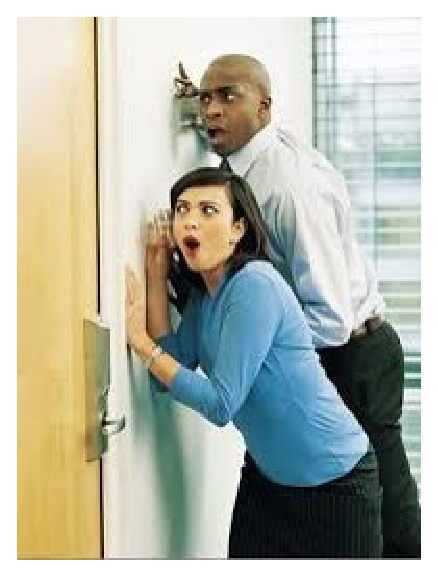
\includegraphics[width=0.28\textwidth]{figures//theme1//Theme1_6.eps}
    }
\end{figure}
}{
\begin{figure}[htbp]
    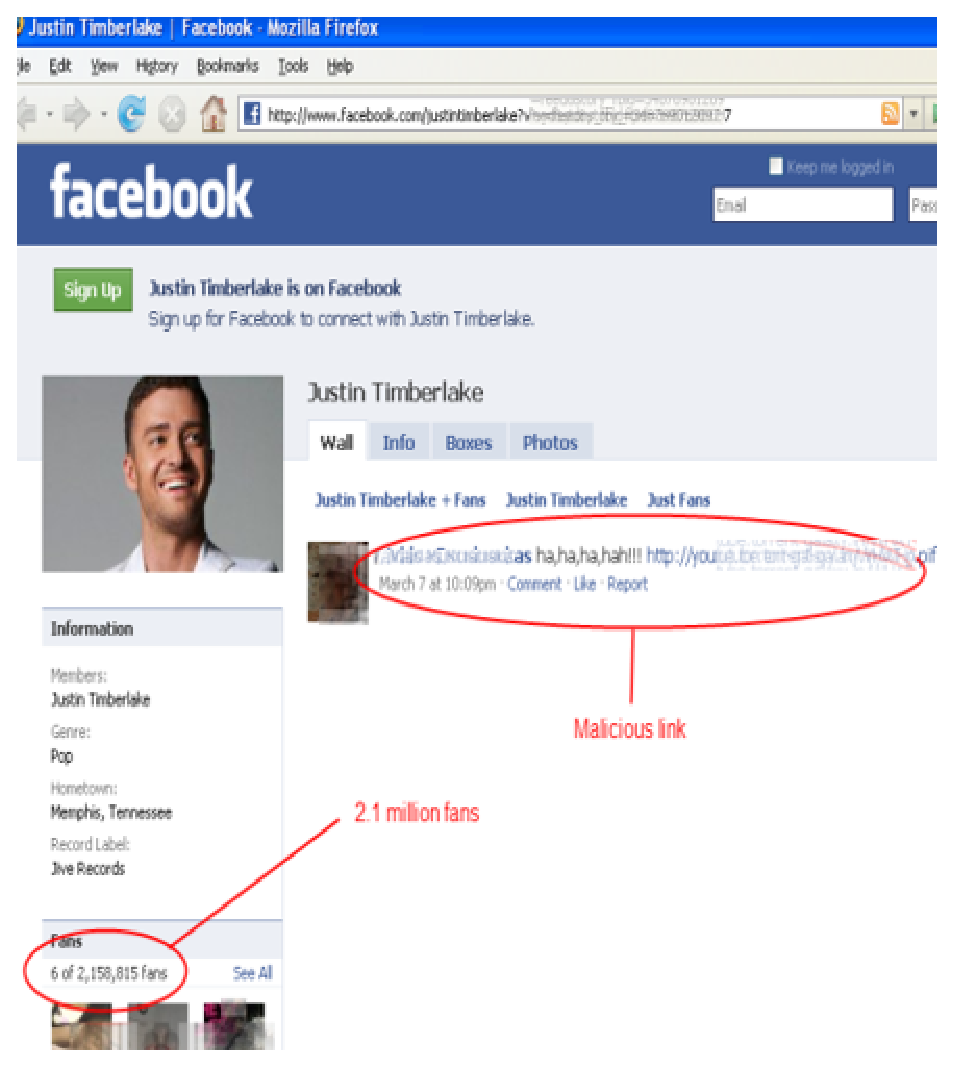
\includegraphics[width=0.7\textwidth]{figures//theme1//Theme1_7.eps}
\end{figure}
}

\end{slide}
%%
%%==========================================================================================


%%==========================================================================================
%%
\begin{slide}[toc=,bm=]{The Popularity of Online Social Networks}

\begin{itemize}
\item
The popularity of OSNs has greatly increased in recent years

\begin{itemize}
\item
A large amount of Internet users also use OSN services,

\item
Australia has up to 11 million Facebook users.
\end{itemize}

\end{itemize}

\begin{figure}[htbp]
    \centering
    \subfigure{
        
\includegraphics[width=0.25\textwidth]{figures//theme1//Theme1_8.eps}
    }
    \subfigure{
        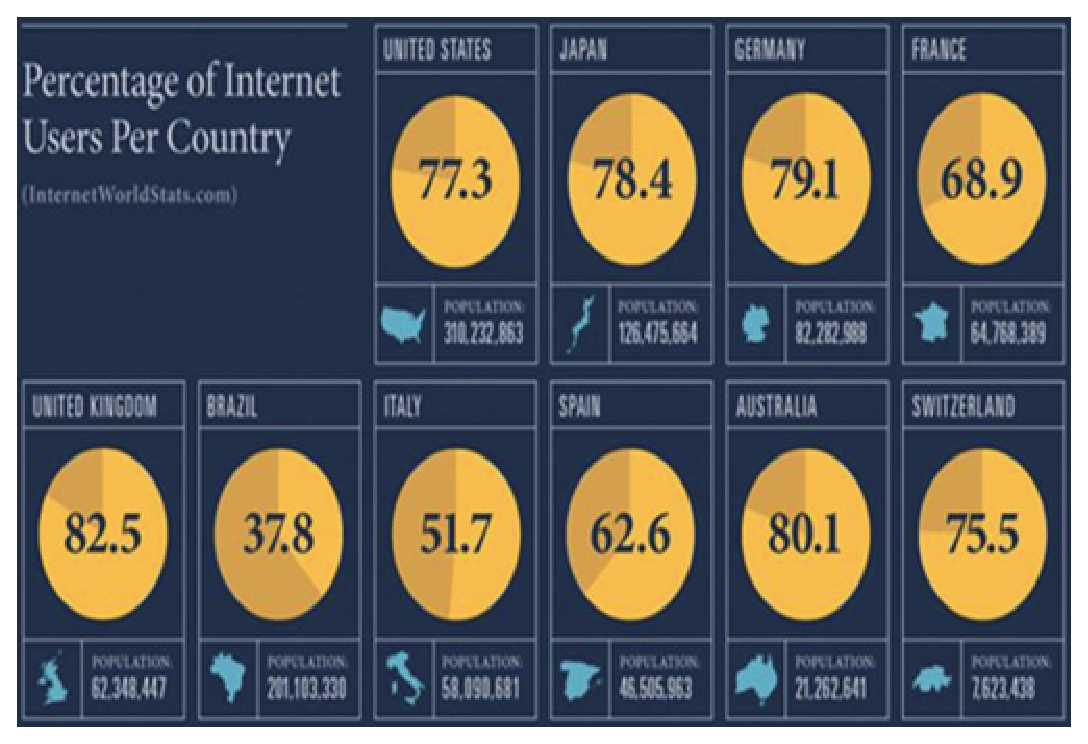
\includegraphics[width=0.37\textwidth]{figures//theme1//Theme1_9.eps}
    }
    \subfigure{
        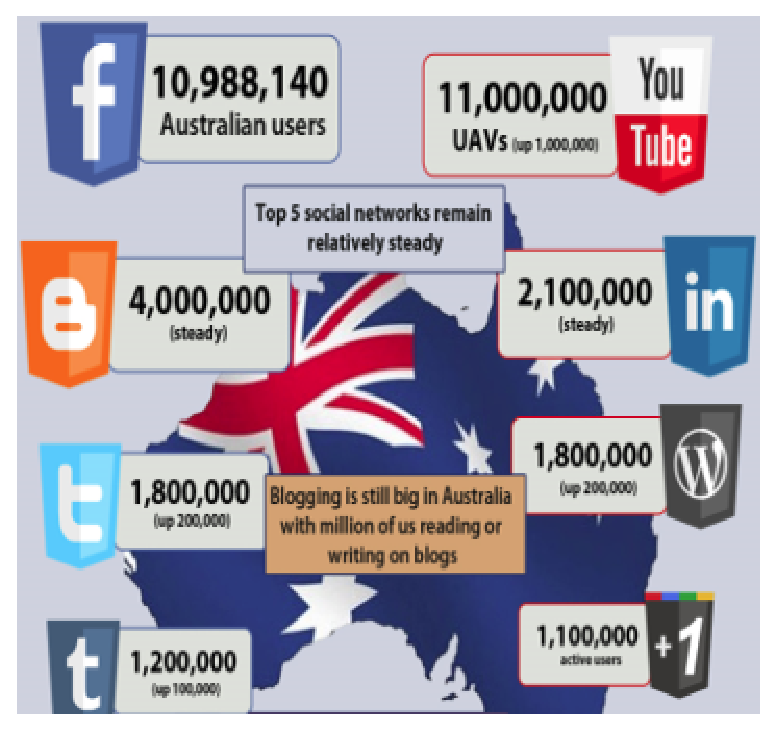
\includegraphics[width=0.3\textwidth]{figures//theme1//Theme1_10.eps}
    }
\end{figure}

\end{slide}
%%
%%==========================================================================================


%%==========================================================================================
%%
\begin{slide}[toc=,bm=]{Application of Geo Photos}

\begin{itemize}
\item
There are many geotagged photos available. However :

\begin{itemize}
\item
Data is noisy or misleading.

\item
Photos are taken in transit rather than at the attractions.

\item
Photo is static media, whereas, travel behavior is dynamic.
\end{itemize}

\end{itemize}
\begin{figure}[htbp]
    \centering
    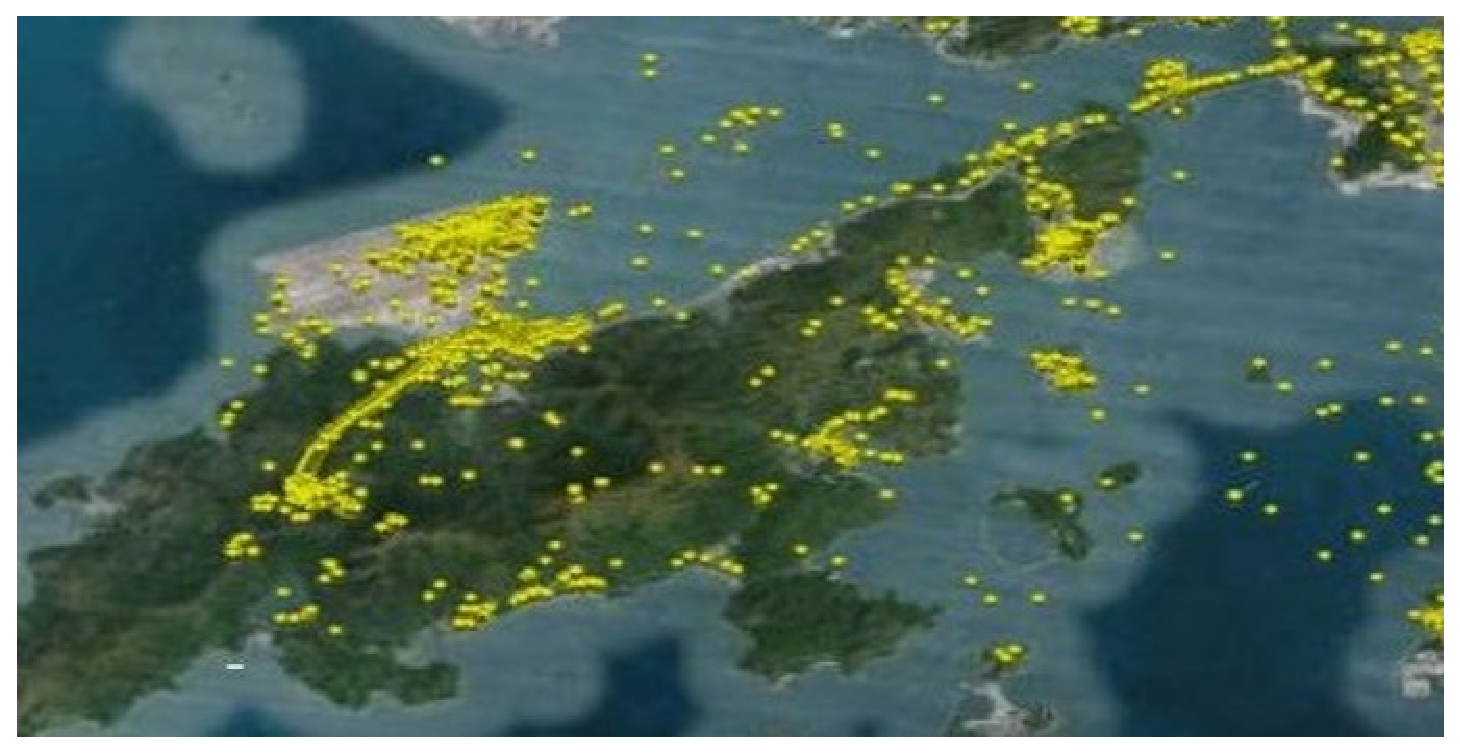
\includegraphics[width=0.5\textwidth]{figures//theme1//Theme1_11.eps}
\end{figure}

\begin{center}
   \onslide{2}{\twotonebox{\huge \textcolor{red}{?}}{\large \emph{How to mine these data for travel behaviour analysis?}}}
\end{center}

\end{slide}
%%
%%==========================================================================================


%%==========================================================================================
%%
\begin{slide}[toc=,bm=]{Tourist Movement Analysis}
Tourist Traffic Flow in Hong Kong Metropolitan Area.

\begin{figure}[htbp]
    \subfigure[Asian Tourist]{
        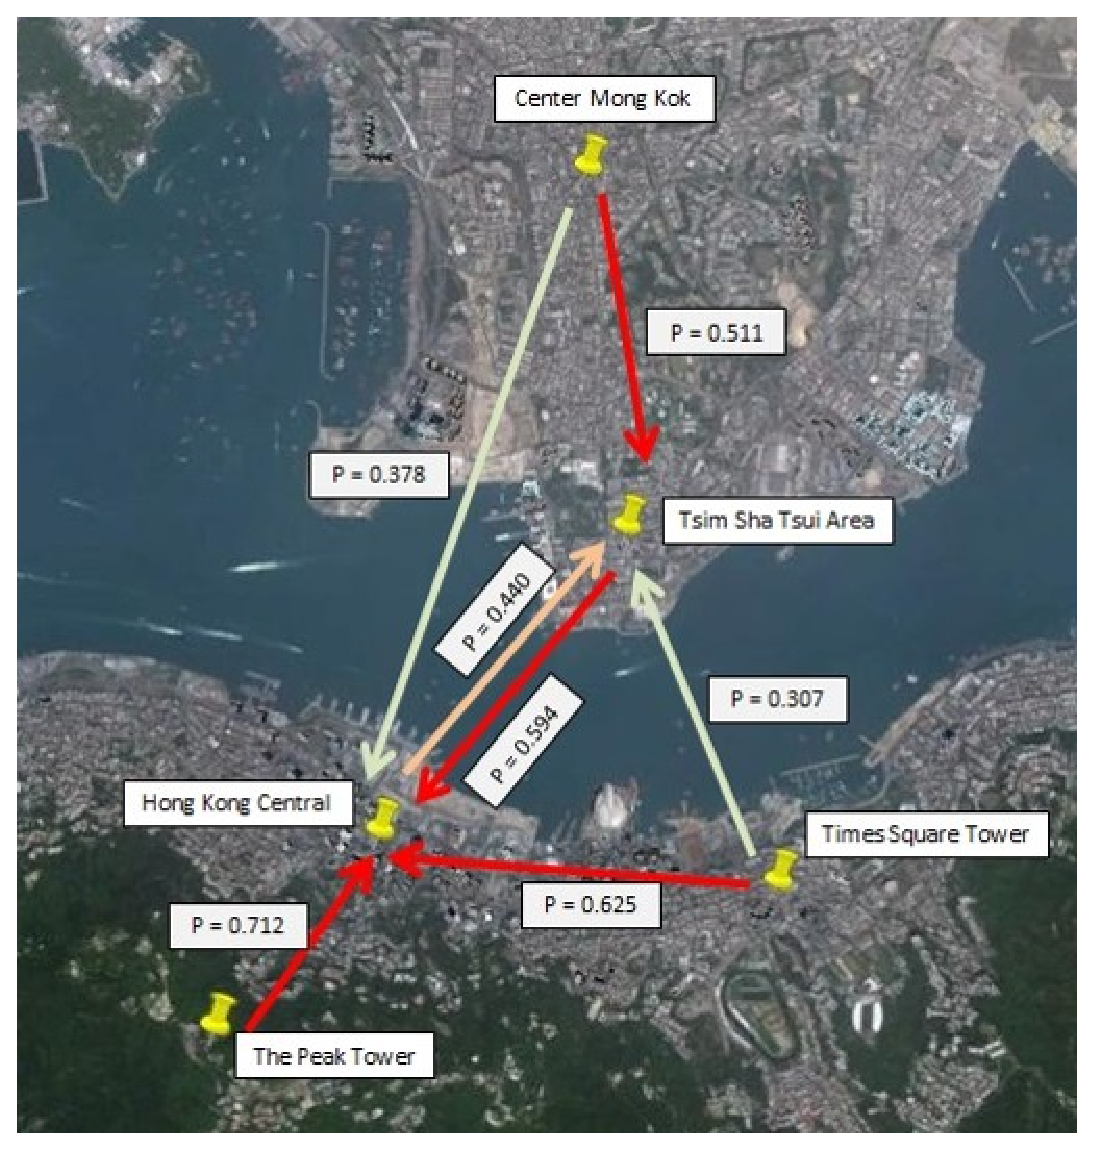
\includegraphics[width=0.4\textwidth]{figures//theme1//Theme1_12.eps}
    }
    \subfigure[Western Tourist]{
        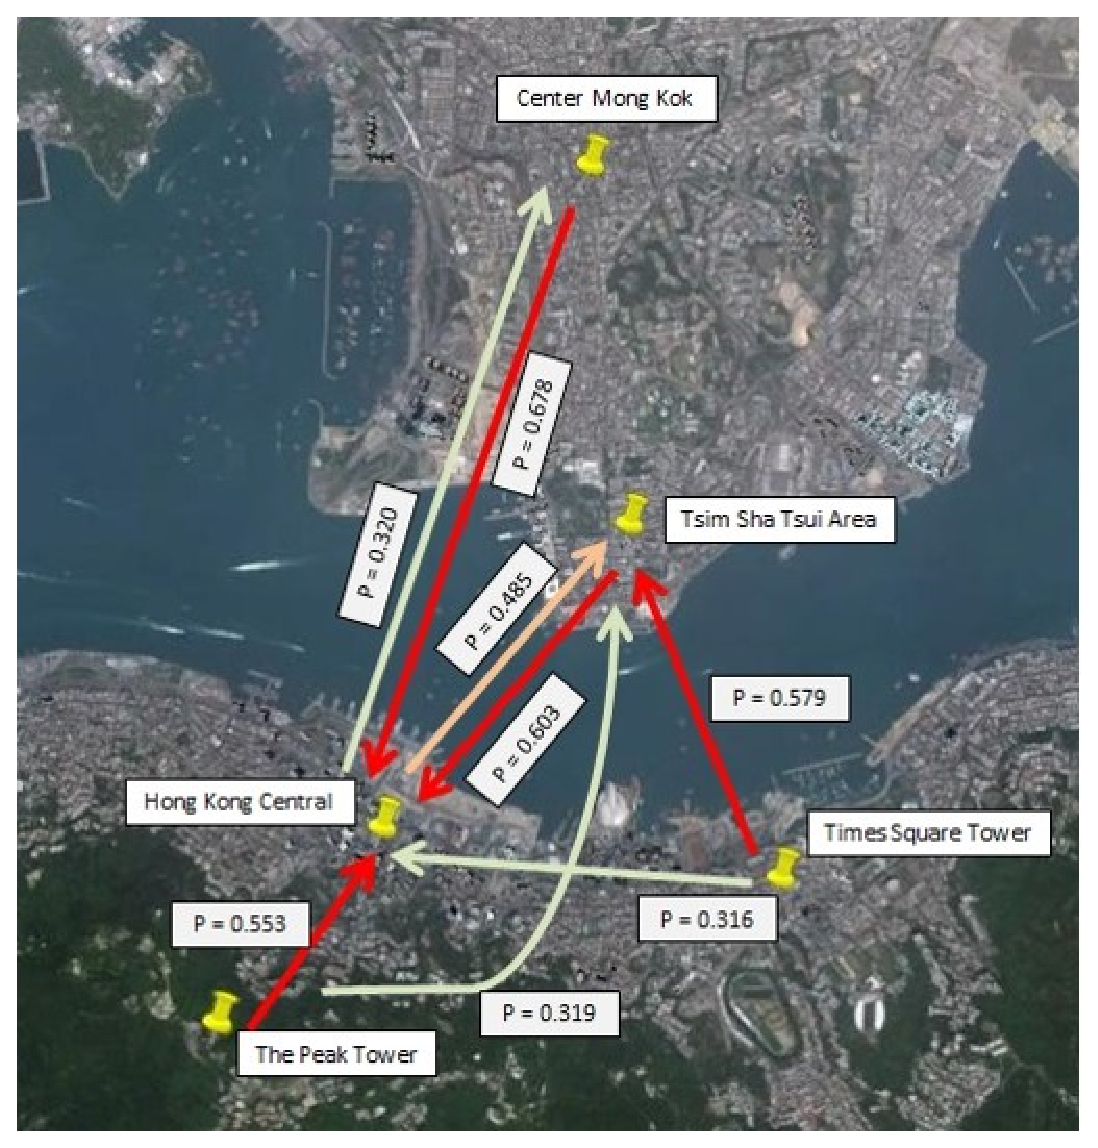
\includegraphics[width=0.4\textwidth]{figures//theme1//Theme1_13.eps}
    }
\end{figure}

\end{slide}
%%
%%==========================================================================================


%%==========================================================================================
%%
\begin{slide}[toc=,bm=]{Tourist Movement Analysis}

\begin{figure}[htbp]
    \subfigure{
        
\includegraphics[width=0.4\textwidth]{figures//theme1//Theme1_14.eps}
    }
    \subfigure{
        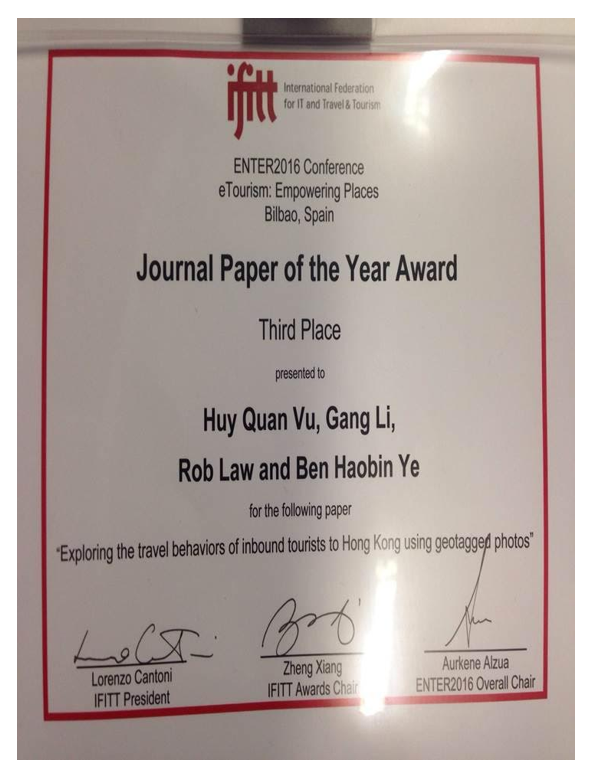
\includegraphics[width=0.2\textwidth]{figures//theme1//Theme1_15.eps}
    }\\
    \subfigure{
        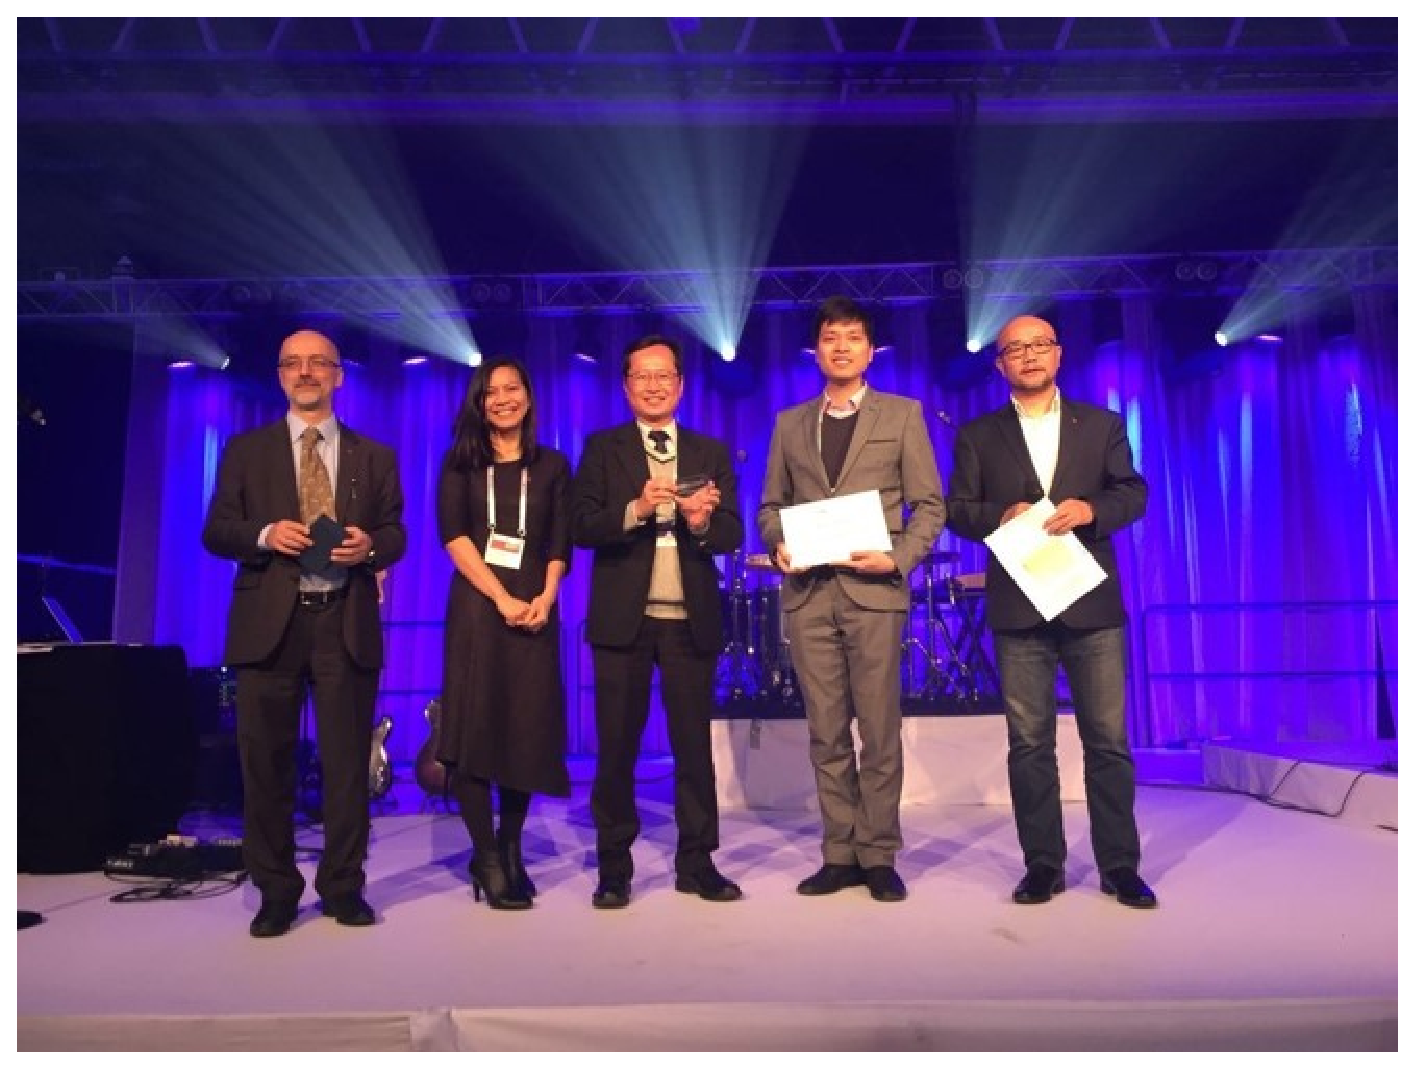
\includegraphics[width=0.3\textwidth]{figures//theme1//Theme1_16.eps}
    }
    \subfigure{
        
\includegraphics[width=0.3\textwidth]{figures//theme1//Theme1_17.eps}
    }
\end{figure}

\footnotesize{Huy Quan Vu, Gang Li, Rob Law, Ben Haobin Yip. 
\emph{Exploring the travel behaviors of inbound tourists to Hong Kong using Geotagged photos. }
Tourism Management.}

\end{slide}
%%
%%==========================================================================================

%%==========================================================================================
%%
\begin{slide}[toc=,bm=]{Periodic Behavior Mining}

\begin{itemize}
\item
Observed Check-in Data is usually a mixed events from different periodic behaviors

\vspace{1cm}

\twocolumn{
\begin{itemize}
\item
What are Periodic?

\item
What is the period?

\item
Predict the Behavior on a particular day.
\end{itemize}}
{
\begin{figure}[htbp]
    \centering
    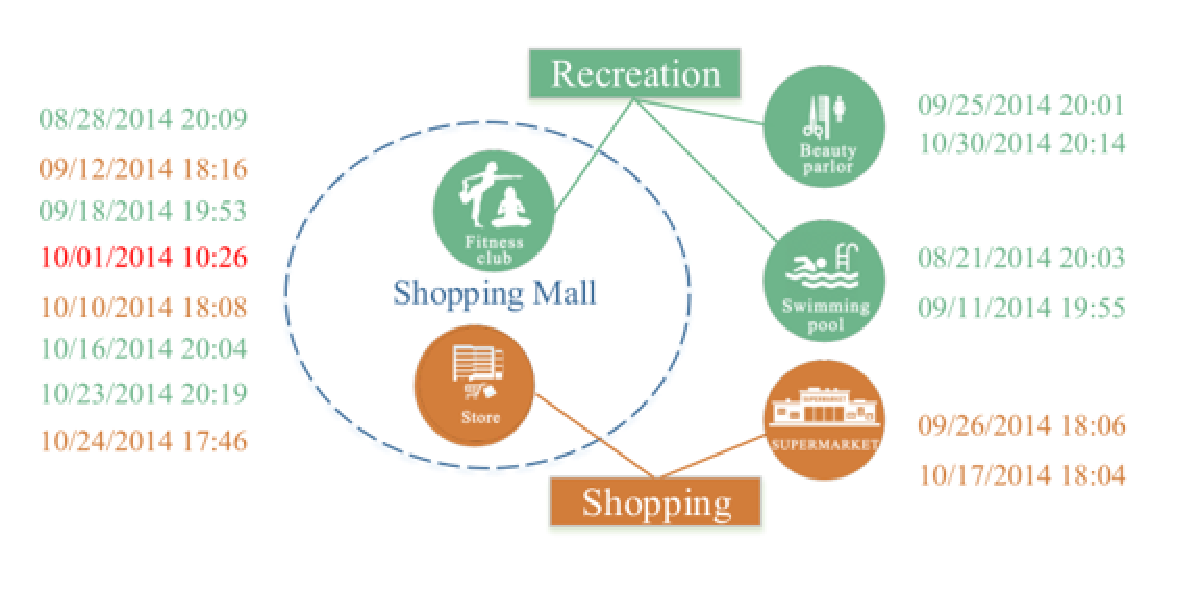
\includegraphics[width=0.9\textwidth]{figures//theme1//Theme1_18.eps}
\end{figure}
}
\end{itemize}




\end{slide}
%%
%%==========================================================================================

%%==========================================================================================
%%
\begin{slide}[toc=,bm=]{Periodic Behavior Mining Mobility Intentions}

\begin{itemize}
\item
CP Decomposition

\end{itemize}

\end{slide}
%%
%%==========================================================================================


%%==========================================================================================
%%
\begin{slide}[toc=,bm=]{Periodic Behavior Mining Applications}

\begin{itemize}
\item
There are various applications of Periodic Behavior Mining

    \begin{itemize}
    \item
    What is the schedule of a person on a particular day/time?

    \item
    Where to find the person on a particular day/time?
        \begin{itemize}
        \item
        Police applications

        \item
        Scheduled ``Encountering'' for match making
        \end{itemize}
    \item
    Timely Recommendation Systems
        \begin{itemize}
        \item
        Now it is the time for you to stock rice, cooking oil, or ice cream!

        \end{itemize}

\end{itemize}

\end{itemize}

\end{slide}
%%
%%==========================================================================================


%%==========================================================================================
%%
\begin{slide}[toc=,bm=]{Data Science Application - Case 1: Face Age Recognition}

\begin{figure}[htbp]
    \subfigure{
        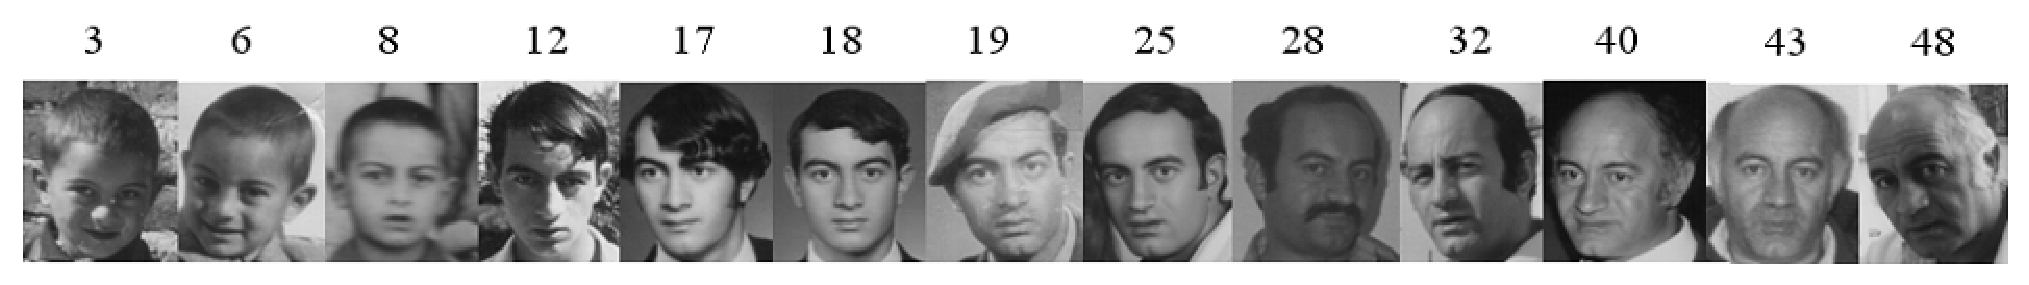
\includegraphics[width=0.8\textwidth]{figures//theme1//Theme1_19.eps}
    }\\
    \subfigure{
        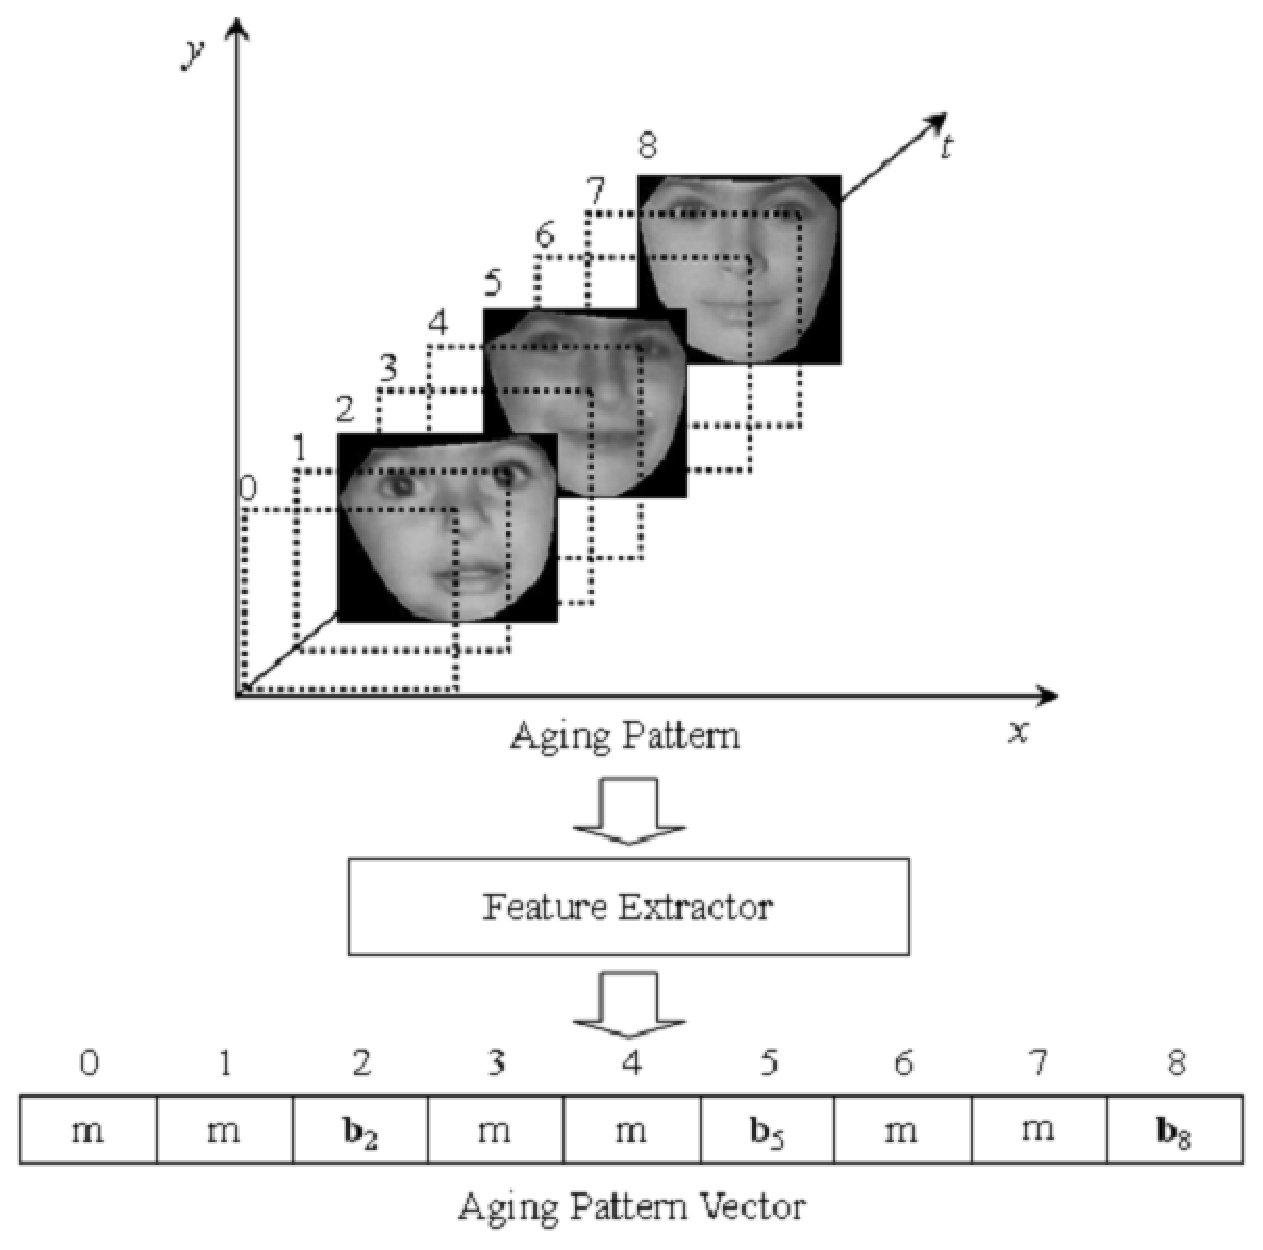
\includegraphics[width=0.3\textwidth]{figures//theme1//Theme1_20.eps}
    }
    \subfigure{
        
\includegraphics[width=0.4\textwidth]{figures//theme1//Theme1_21.eps}
    }
\end{figure}

\footnotesize{Xin Geng, Zhi-Hua Zhou, Yu Zhang, Gang Li, Honghua Dai.
\emph{Learning from facial aging patterns for automatic age estimation. }
Proceedings of the 14th annual ACM international conference on Multimedia, 2006}

\end{slide}
%%
%%==========================================================================================


%%==========================================================================================
%%
\begin{slide}[toc=,bm=]{Data Science Application - Case 2: Speech-based Emotion Detection}

\begin{figure}
  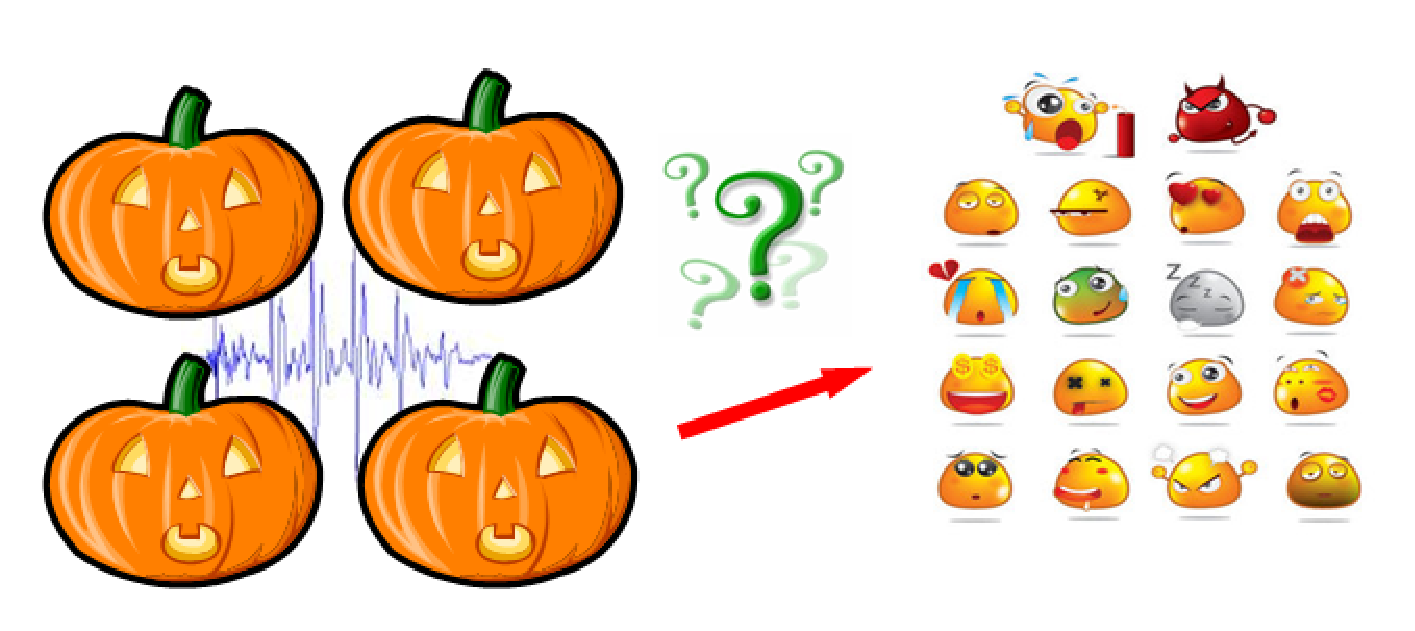
\includegraphics[width=0.8\textwidth]{figures//theme1//Theme1_22.eps}
\end{figure}

\footnotesize{Jia Rong, Gang Li, Yi-Ping Phoebe Chen.
\emph{Acoustic Feature Selection for Automatic Emotion Recognition from Speech. }
Information Processing and Management, 45(3):  315-328 2009
}

\end{slide}
%%
%%==========================================================================================


%%==========================================================================================
%%
\begin{slide}[toc=,bm=]{Data Science Application - Case 3: K-Complex Detection}


\end{slide}
%%
%%==========================================================================================


%%==========================================================================================
%%
\begin{slide}[toc=,bm=]{Data Science Application - Case 4: Trajectory Analysis}


\end{slide}
%%
%%==========================================================================================


%%==========================================================================================
%%
\begin{slide}[toc=,bm=]{Data Science Application - Case 5: Video Surveillance}
\begin{figure}[ht]
  \includemovie[poster=figures//theme1//Theme1_23.eps,
  inline=false,
%  text={\small(Loading Video Surveillance.avi)}
  ]
  {12cm}{11cm}{figures//theme1//Video Surveillance.avi}
\end{figure}
%\begin{figure}
%  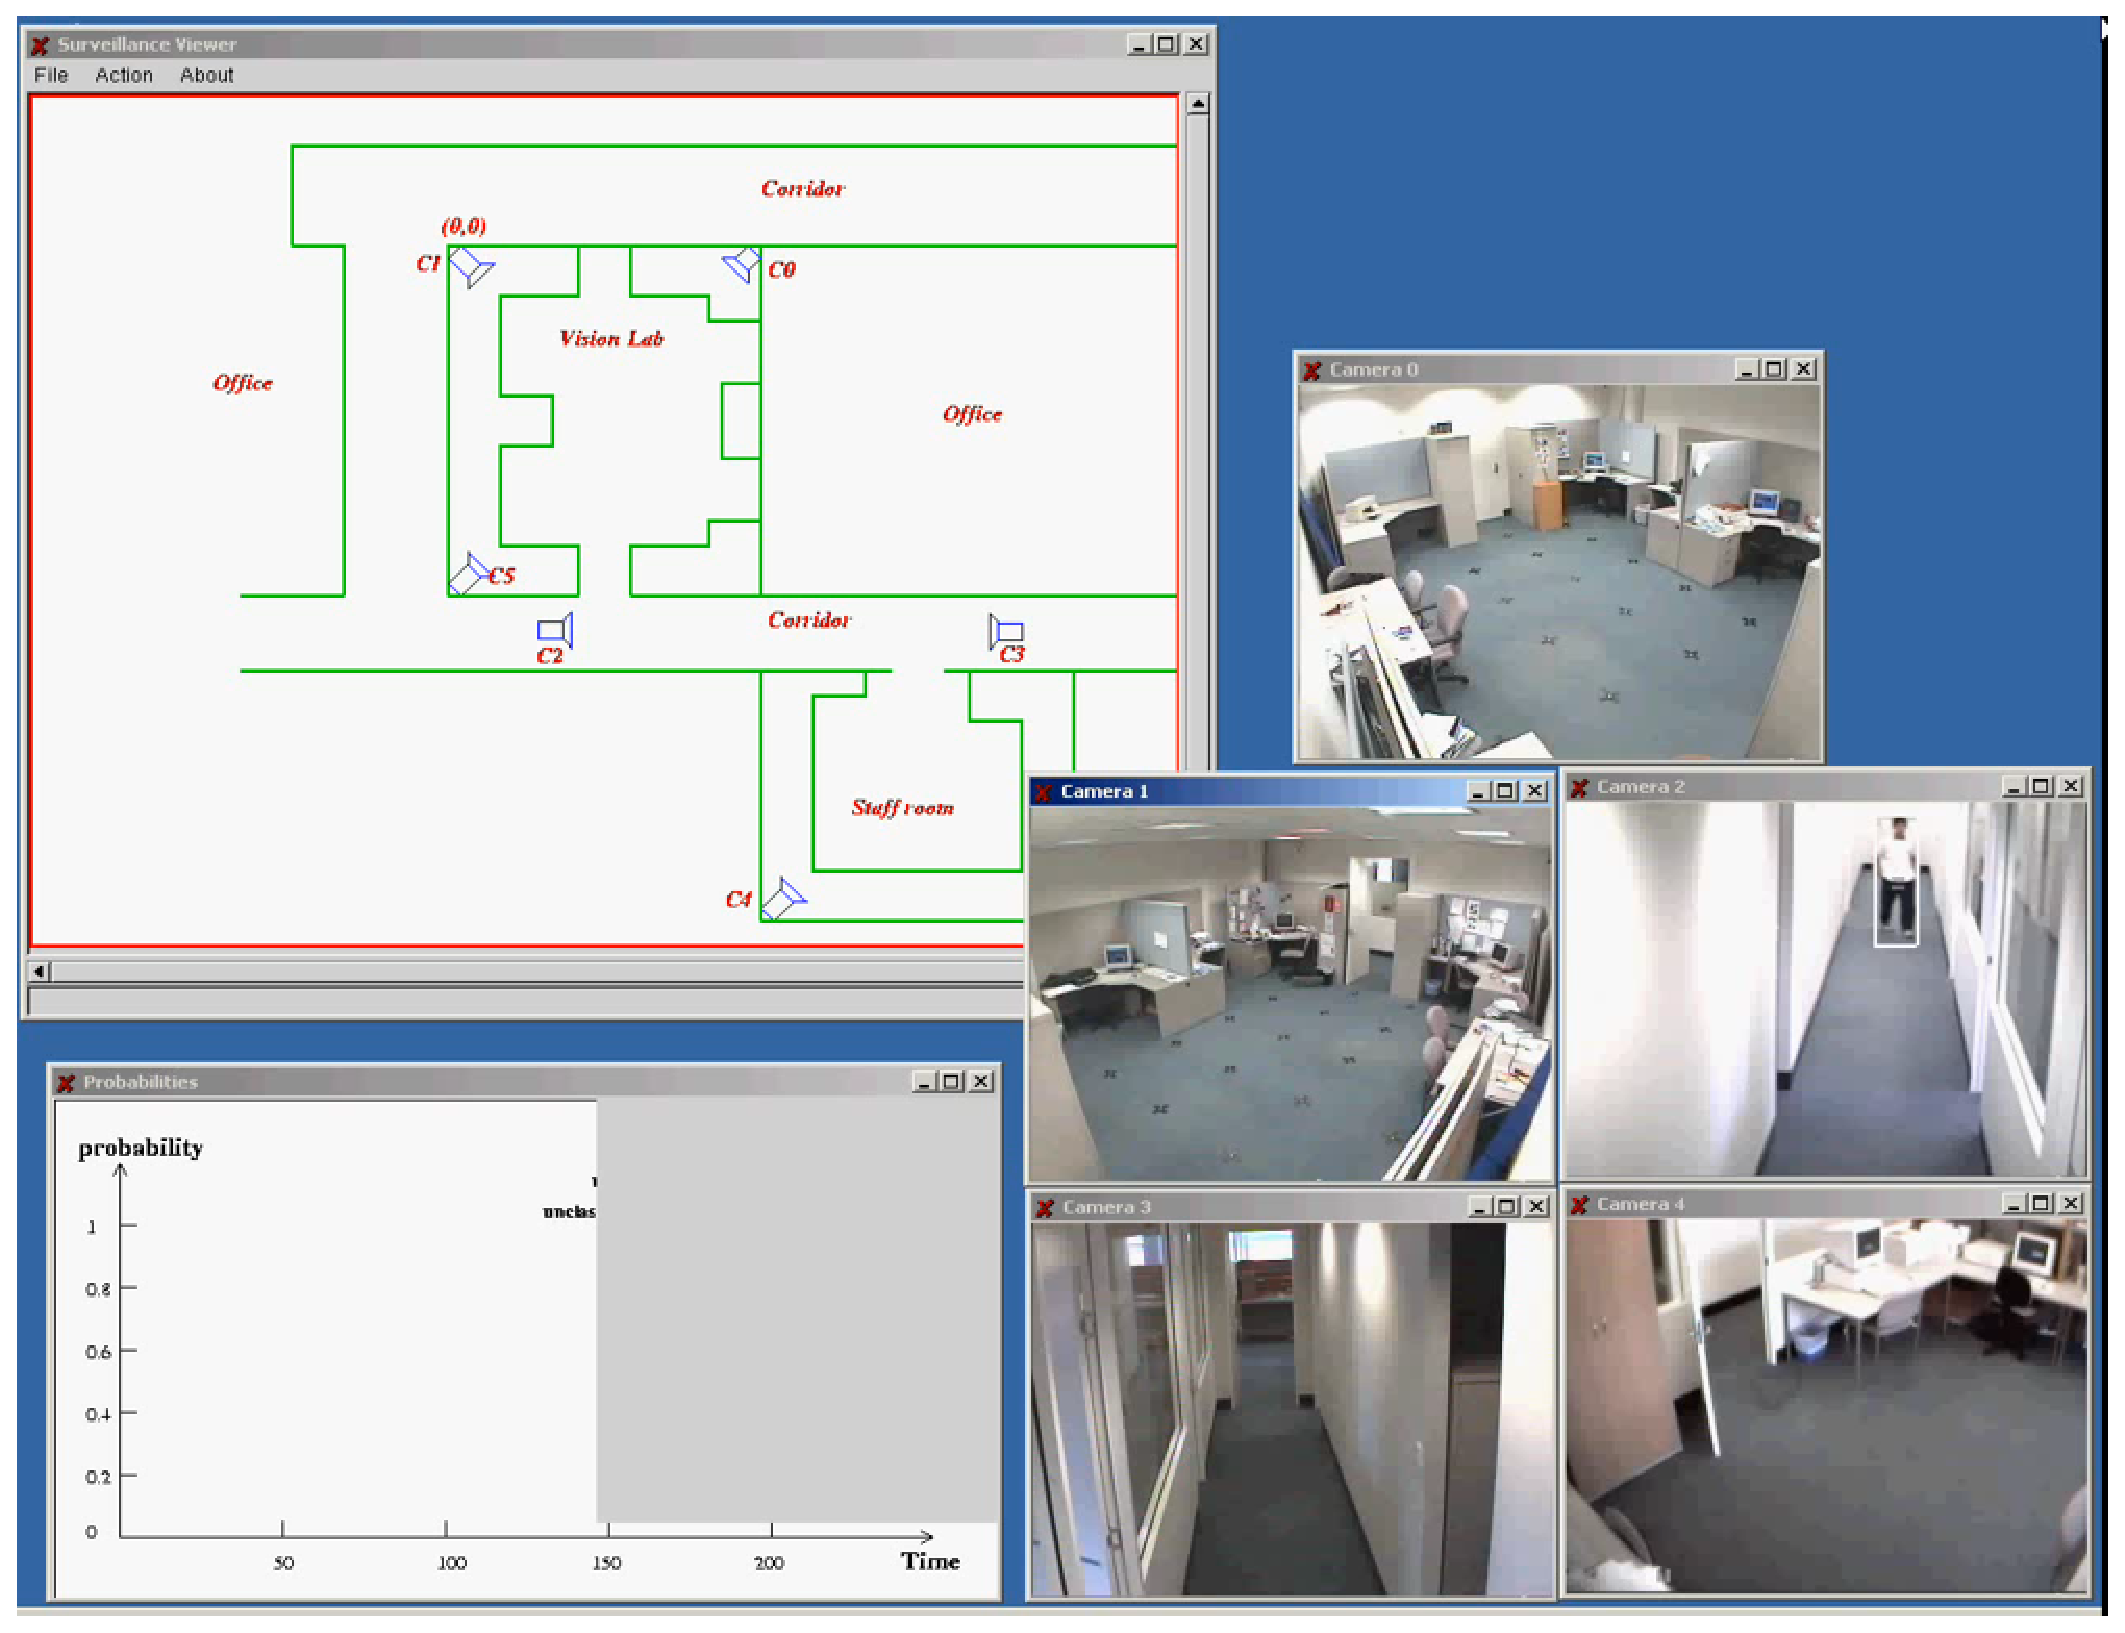
\includegraphics[width=0.7\textwidth]{figures//theme1//Theme1_23.eps}
%\end{figure}

\end{slide}
%%
%%==========================================================================================

%%==========================================================================================
%%
\begin{slide}{Theme 2. Information Abuse Prevention}
%Theme two -
\begin{itemize}
\item
Information Abuse:


\begin{itemize}
\item
The compromise of information
for which the data stakeholders are not willing to disclose.


\item
It depends on the nature of the information,
the involved internal or external users,
and the ways in which the organization grants the access to
or releases the information.

\end{itemize}
\end{itemize}

\end{slide}
%%
%%==========================================================================================


%%==========================================================================================
%%
\begin{slide}[toc=,bm=]{Who is an adversary?}

\begin{itemize}
\item
Every user is potentially an adversary

\begin{itemize}
\item
After data is released, we cannot prevent any user from performing any type of analysis on the released data

\item
Worst case scenario

\begin{itemize}
\item
Must account for disclosure risk from any and all types of analyses
\end{itemize}

\end{itemize}
\end{itemize}

\end{slide}
%%
%%==========================================================================================


%%==========================================================================================
%%
\begin{slide}[toc=,bm=]{Information Privacy Applications - Case 1: Privacy Breach}

\end{slide}
%%
%%==========================================================================================


%%==========================================================================================
%%
\begin{slide}[toc=,bm=]{Information Privacy Applications - Case 2: Privacy Breach}


\end{slide}
%%
%%==========================================================================================


%%==========================================================================================
%%
\begin{slide}[toc=,bm=]{Information Privacy Applications - Case 3: Is O.S.N. a Secure Place to Show off?}


\end{slide}
%%
%%==========================================================================================

%%==========================================================================================
%%
\begin{slide}[toc=,bm=]{Privacy Preserving Related Reference}


\end{slide}
%%
%%==========================================================================================

%%==========================================================================================
%%
\begin{slide}[toc=,bm=]{Theme 3. Business Intelligence}

\begin{itemize}
\item
Tourism Data Mining

\begin{itemize}
\item
Tourist Behavior Analysis

\item
Contrast Mining

\begin{itemize}
\item
Outlying Aspects Mining

\item
Competitiveness Discovery
\end{itemize}

\end{itemize}

\item
Recommendation System

\end{itemize}

\end{slide}
%%
%%==========================================================================================


%%==========================================================================================
%%
\begin{slide}[toc=,bm=]{Business Intelligence Applications \\
\small{Case 1: Market Segmentation Analysis}}


\end{slide}
%%
%%==========================================================================================


%%==========================================================================================
%%
\begin{slide}[toc=,bm=]{Business Intelligence Applications - Case 2: Negative Association Rule Mining}


\end{slide}
%%
%%==========================================================================================


%%==========================================================================================
%%
\begin{slide}[toc=,bm=]{Business Intelligence Applications - Case 3: Contrast Mining}


\end{slide}
%%
%%==========================================================================================


%%==========================================================================================
%%
\begin{slide}[toc=,bm=]{Business Intelligence Applications - Case 4: Heterogeneous Preferences}

\begin{itemize}
\item
User-wise biases

\begin{itemize}
\item
Users give lower ratings when in bad mood

\item
Different scales, e.g., 4/5 star is ``OK'' for critics

\item
User interface design

\end{itemize}

\item
Item-wise biases

\begin{itemize}
\item
The same item presented differently,
e.g., a movie in 3D, HD

\end{itemize}
\end{itemize}
\end{slide}
%%
%%==========================================================================================


%%==========================================================================================
%%
\begin{slide}[toc=,bm=]{Business Intelligence Applications - Case 5: PR-based Conditional Random Fields}


\end{slide}
%%
%%==========================================================================================

%%==========================================================================================
%%
\begin{slide}[toc=,bm=]{Our rankings}


\end{slide}
%%
%%==========================================================================================

%%==========================================================================================
%%
\begin{slide}[toc=,bm=]{Awards}


\end{slide}
%%
%%==========================================================================================


\section{Training at TULIP}


%%==========================================================================================
%%
\begin{slide}{Training at TULIP}
\begin{itemize}
  \item \textcolor{orange}{Professional knowledge}
    \begin{itemize}
          \item \LaTeX{},
                Version Control System (\texttt{SmartGit Github Bitbucket})
          \item Plan \& Progress Review
          \item References Management
        \end{itemize}
  \item \textcolor{orange}{Foundational Knowledge}
    \begin{itemize}
      \item FLIP (00)\texttildelow FLIP (05)
    \end{itemize}
  \item \textcolor{orange}{Research Skills}
    \begin{itemize}
      \item Review Team
      \item Reading Team
        \begin{itemize}
          \item QQ Online
          \item At least once a month
          \item Read material before meeting,
                ask questions.
        \end{itemize}
    \end{itemize}
\end{itemize}

\end{slide}
%%
%%==========================================================================================


\begin{slide}[toc=,bm=]{Training at TULIP}
    \begin{itemize}
      \item Learning content (FLIP (00)\texttildelow FLIP (05))
        \begin{enumerate}
          \item \textcolor{orange}{Mathematics}
            \begin{itemize}
              \item Linear algebra,
                    Probability theory,
                    Mathematical statistics
            \end{itemize}
          \item \textcolor{orange}{Hand-on Skills}
            \begin{itemize}
              \item Python,
                    Apache Spark,
                    Cloud platform
            \end{itemize}
          \item \textcolor{orange}{Learning theoretical knowledge}
            \begin{itemize}
              \item Optimization,
                    Graph model
            \end{itemize}
          \item \textcolor{orange}{Professional Knowledge}
        \end{enumerate}
    \end{itemize}
\end{slide}




\begin{slide}[toc=,bm=]{Training at TULIP}
\begin{center}

\selectcolormodel{rgb}
   \begin{tikzpicture}[ every annotation/.style = {draw,
                     fill = white}]
  \path[mindmap,concept color=black!40,text=white,
    every node/.style={concept},
    root/.style    = {concept color=black!40,
      font=\Large\bfseries,text width=10em},
    level 1 concept/.append style={font=\bfseries,
      sibling angle=100,text width=7.7em,level distance=8em,inner sep=0pt},
    level 2 concept/.append style={font=\sf,text width=5em,inner sep=0pt},
  ]
  node[root,scale=0.6] {Training at TULIP} [clockwise from=180]
    child[concept color=blue!60] {
      node[scale=0.6] {Professional knowledge} [clockwise from=260]
        child { node[scale=0.6] {\LaTeX} }
        child { node[scale=0.6] (goReview) {Plan \& Progress Review }}
        child { node[scale=0.6] (goRefrences ){References Management}}
        child { node[scale=0.6] (goVersionCon) {Version Control System}}
    }
     child[concept color=blue] {
      node[concept,scale=0.6] {Foundation (FLIP(00-05))}[clockwise from=160]
      child{node[concept,scale=0.6](hand-on){Hand-on Skills}}
      child{node[concept,scale=0.6](Professional){Professional Knowledge}}
      child{node[concept,scale=0.6](Theo){Theoretical knowledge}}
      child{node[concept,scale=0.6](Math){Mathmatics}}
    }
    child[concept color=orange] {
      node[concept,scale=0.6] {Research Skills}
        [clockwise from=60]
      child { node[concept,scale=0.6] (TeXampleBlog)
        {Reading Team} }
      child { node[concept,scale=0.6] (Reviewteam)
        {Review Team }}
    }
   ;
    \info{Reviewteam.north east}{above,anchor=west,xshift=0.5em}{%
      \item QQ Online
      \item At least once a month
      \item Read material before meeting
      \item Ask questions.
    }
    \info{goVersionCon.north west}{above,anchor=east,xshift=-0.5em}{%
      \item SmartGit
      \item GitHub
      \item Bitbucket
    }
    \info{Math.north east}{above,anchor=west,xshift=0.5em}{%
      \item Linear algebra
      \item Probability theory
      \item Mathematical statistics
    }
    \info{hand-on.north west}{above,anchor=east,xshift=-0.5em }{
      \item Python
      \item Apache Spark
      \item Cloud platform
    }
    \info{Theo.north east}{above,anchor=west,xshift=0.5em}{
      \item Optimization
      \item Graph model
    }
    \end{tikzpicture}
\end{center}
\end{slide}

\begin{slide}{Aiming Higher \dots}
    \begin{itemize}
      \item \textcolor{orange}{TULIP Academy:}
       \begin{enumerate}
         \item Complete FLIP (00)\texttildelow FLIP (01) with test on Kaggle Project;
         \item Read materials before TULIP Seminar and ask questions;
         \item Learn \LaTeX{} \& PPR.
       \end{enumerate}
       \begin{itemize}
         \item \textcolor{orange}{Trainee:}
         \begin{enumerate}
           \item Complete  FLIP (02)\texttildelow FLIP (03) with Kaggle
           \item Report in TULIP Seminar
           \item SmartGit, Bitbucket and Mendeley
         \end{enumerate}
         \begin{itemize}
           \item \textcolor{orange}{Infinity:}
            \begin{enumerate}
              \item Meeting with Gang Leader twice a week (Research)
              \item Complete  FLIP (04)\texttildelow FLIP (05)
            \end{enumerate}
         \end{itemize}
       \end{itemize}

    \end{itemize}
\end{slide}


\section{Rules in TULIP}


%%==========================================================================================
%%
\begin{slide}{Regulations}

\begin{center}
\begin{itemize}

\item<1->
{TULIP Academy}

\begin{itemize}
\item
You must not be absent from the meeting without permission.

\item
Xi'an group members must attend the seminar in the Lab,
and NOT online.

\item
Collaborate with team members, rather than attacking each other.
\end{itemize}

\item<2->
{FLIP Study}

\begin{itemize}
\item
All FLIP students need to pass the corresponding prerequisite.

\item
All FLIP materials are confidential, and you should not circulate it outside.
\end{itemize}

\item<3->
{Research}

\begin{itemize}
\item
\texttt{SmartGit}, \texttt{Bitbucket}, \texttt{Mendeley},
update PPR in time.

\item
Actively discuss research work in the group meeting, and TULIP Seminar.

\item
Everyone should prepare at least one question for each TULIP seminar.
\end{itemize}
\end{itemize}
\end{center}

\end{slide}
%%
%%==========================================================================================


%%==========================================================================================
%
\begin{slide}[toc=,bm=]{Questions?}

\vspace{4.5cm}
\begin{center}
{\twotonebox{\Huge ?}
{\large \emph{Any Questions}}}
\end{center}

\end{slide}
%%
%%==========================================================================================


%%==========================================================================================
% TODO: Contact Page
\begin{wideslide}[toc=,bm=]{Contact Information}
\centering
\vspace{\stretch{1}}
\twocolumn[
lcolwidth=0.35\linewidth,
rcolwidth=0.65\linewidth
]
{
% \centerline{
\includegraphics[scale=.2]{tulip-logo.eps}}
}
{
\vspace{\stretch{1}}
Associate Professor \emph{Gang Li}\\
School of Information Technology\\
Deakin University, Geelong, Australia
\begin{description}
 \item[Email] \href{mailto:gangli@acm.org}
 {\textsc{\footnotesize{gangli@acm.org}}}

 \item[Lab] \href{http://www.tulip.org.au}
 {\textsc{\footnotesize{Team for Universal Learning and Intelligent Processing}}}
\end{description}
}
\vspace{\stretch{1}}
\end{wideslide}

\end{document}

\endinput
